\Chapter{Kiterjesztett és virtuális valóság}

\begin{itemize}
\item[AR] (\textit{Augmented Reality}):
A kiterjesztett vagy augmentált valóság alatt a valóság kibővítését értjük. Ehhez valamilyen eszköz kameráján keresztül kell szemlélnünk a teret.
\item[VR] (\textit{Virtual reality}): A virtuális valóság, a valóság teljes kizárása és egy virtuális környezetbe kerülést jelent. 
\item[MR] (\textit{Mixed Reality}): az AR és VR keveréke, a valós teret bővíti ki, ahogy az AR, azonban itt a cél a virtuális és valós környezet határának elmosása, nagyobb hangsúlyt kap az interakció. 
\end{itemize}

\Section{Hardware}

\SubSection{AR hardware}

Ahhoz, hogy ízelítőt kapjuk a kiterjesztett valóság használatának élményéből elegendő egy megfelelő operációs rendszerrel rendelkező mobiltelefon, tablet. ( Android 7 és annál újabb, iOs 11 és újabb)
Számos alkalmazás, játék eléhető, amik nem igényelnek speciális eszközöket. 

Ezek az okos eszközök azért felelnek erre a célra, mert rendelkeznek kamerával ( a legújabb telefonok már igen éles és tiszta képet adnak) és olyan szenzorokkal, amik  szükségesek.

Ezen érzékelők  mikro-elektromechanikai (MEMS, \textit{MicroElectroMechanical Systems}) 
rendszerek, azaz olyan apró (karakterisztikus méretük jellemzően 20\-1000 mikrométer) rendszerek amelyek mechanikai és elektronikai alkatrészeket is tartalmaznak.

A telefonok a következő MEMS szenzorokat tartalmazzák:
\begin{itemize}
\item {\bf Inerciális szenzor}: accelerometer és giroszkóp együttese.
\item {\bf Gyorsulásérzékelő} (accelerometer) : „ A gyorsulásmérő gyorsulás mérésére szolgáló műszer. Mivel azonban a gyorsulást közvetlenül nehéz(kes) mérni, ezért az ilyen műszer a gyorsuláskor fellépő erőt méri, ami Newton 2. törvényének megfelelően: $F = m\cdot a.$"

\item {\bf Giroszkóp}: „A szögelfordulás és szögsebesség mérésére szolgáló eszköz.”
\item Fontos érzékelő még a távolságérzékelő, iránytű, fényváltozás érzékelő.
\end{itemize}

Az asztali számítógépek valamint laptopok is használhatók erre a célra, ha el vannak látva kamerával.

A Unity legújabb verziói (2019.3-tól sé annál frissebb) már nem csak a Windows-t és MacOS támogatják, hanem  lehetővé teszik a Linux operációs rendszerekre való fejlesztést is.

Emellett számos speciális, kifejezetten erre a célra fejlesztett eszköz elérhető, 2019 legnépszerűbb darabjai a következők:
\begin{itemize}
\item {\bf Microsoft Hololens 2} egy olyan vezeték nélküli AR headset, ami két 2k-s 120Hz-ces kijelzővel rendelkezik, ami jobb felhasználói élményt bíztosít, mint a versenytársai. Számos mikrofonnal, egy HD kamerával és fényérzékelővel fel szerelve a Holographic Processing Unit mellett, ami a felhasználó és a virtuális világ közötti interakciót biztosítja..
\item A {\bf MagicLeap One} futurisztikus kinézettel rendelkező AR headset, amit egy Lightpack nevű apró számítógép vezérel, ami elfér az ember zsebében.  A Hololens-hez hasonlóan nem csak kivetít egy képet a valós képre, hanem bizonyos fokú interakciót is lehetővé tesz. A különbség az interakció módjában rejlik, ugyanis a MagicLeap a szem és kéz mozgás követése helyett kontrollerrel rendelkezik.
\item Az {\bf Epson Moverio} kifejezetten munkára tervezetett AR headset, robosztus kialakítása van. Az Epson Moverio által használt Si-Oiled technológia tiszta, éles képet bíztosít. Egy Intel Axom 3 processzor hajtja és Android 5.1 használ.  Alkamlas drón írányításhoz, ami a szem mozgását követve nevigálja magát.
\item A {\bf Google Glass Enterprise} verziója nem igényel kontrollert, kéz nélkül használható.
Az Enterprise plussz funkciói a többi Googke Glass-hoz képest:
\begin{itemize}
\item hangvezérlés
\item könnyebb súly
\item hosszabb akkumulátor élettartam
\item gyorsabb processzor és 8Mp kamera.
\end{itemize}
\end{itemize}

\begin{figure}[htp]
    \centering
   	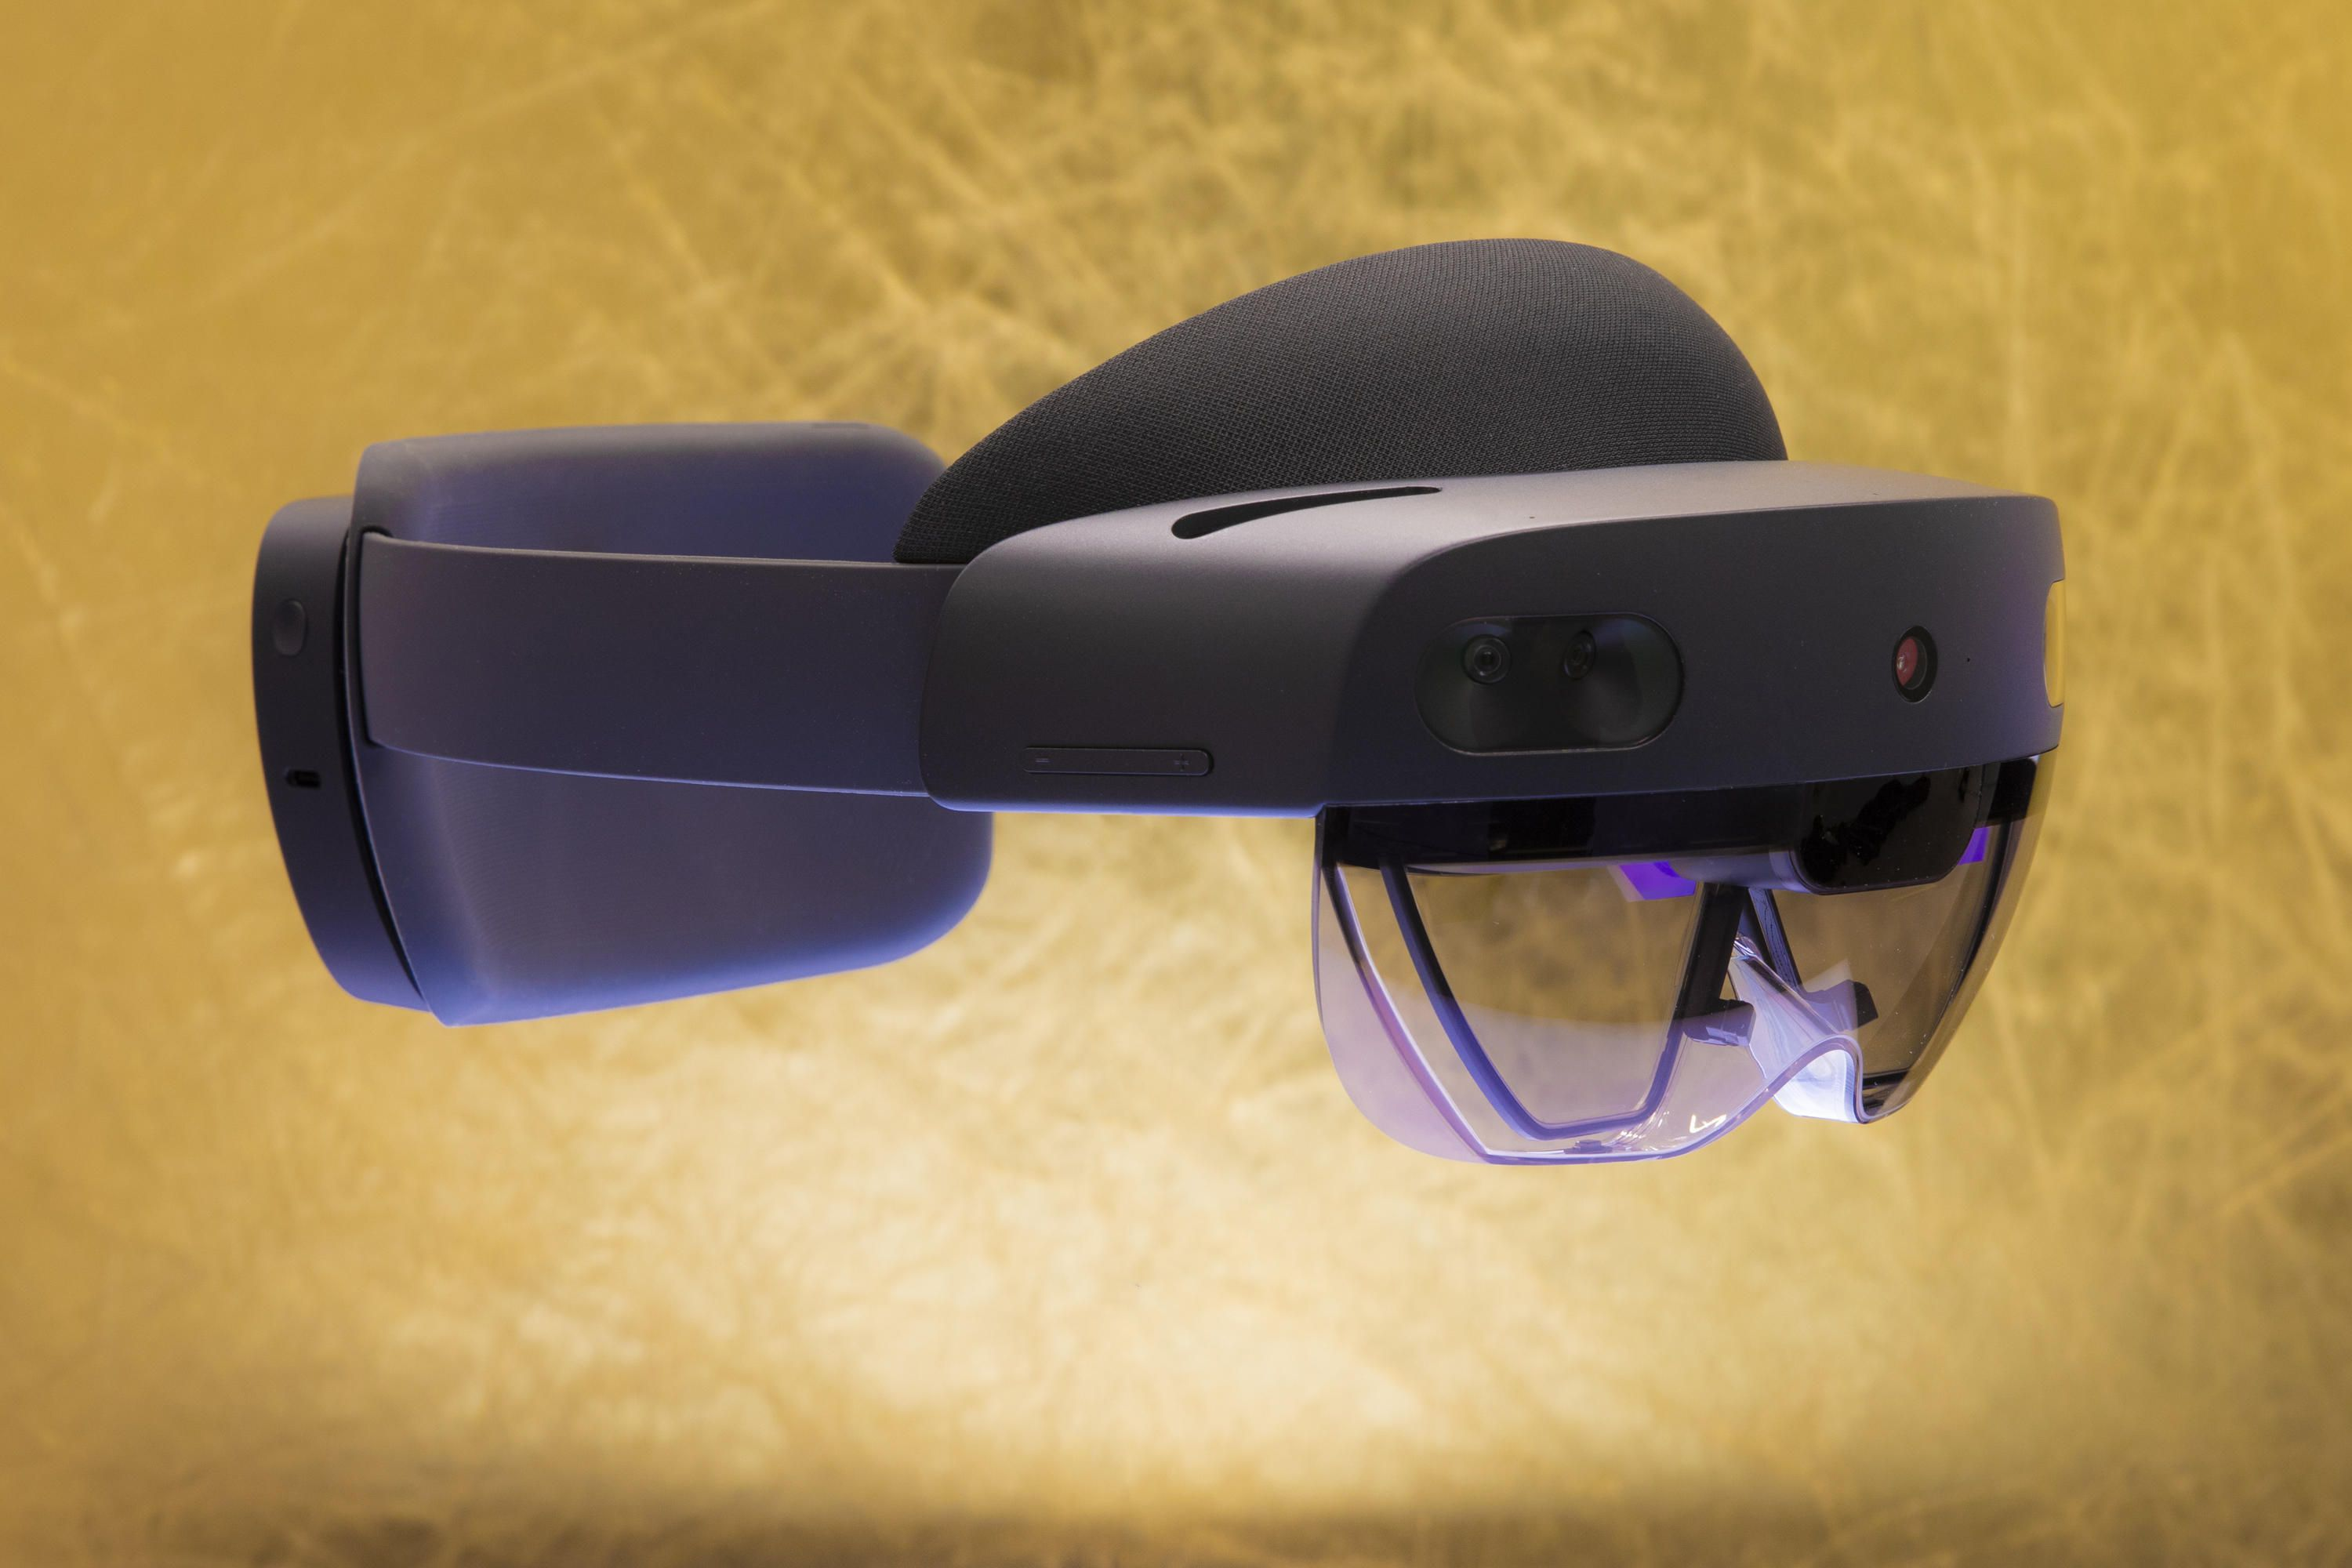
\includegraphics[width=5truecm, height=3.8truecm]{images/holo.jpg}
	\caption{Hololens 2 Ar szemüveg}
\end{figure}

Azonban ezeknek az eszközöknek magas áruk van. 

\SubSection{VR hardware}

A virtuális tér kialakításához szükség van megfelelő hardwarekre (hangrenszer, kijelző (VR szemüveg), számítógép, telefon, konzol) szenzorokra, amik követik a felhasználó mozgását (test, kéz, fej)

{\bf 2020\- ban a legjobb VR headseatek:}
\begin{itemize}
\item Valve Index : remekül működik régebbi GPU esetén is, éles kijelzővel rendelkezik és a Valve kontroller képes az összes új mozgását követni. Azonban nehéz kalibrálni és beállítani. Drága és nehéz hozzájutni.
\item Oculus Quest 2: standalone, könnyű a használata, azonban Facebook fiók hozzáadást igényel.
\item PlayStation VR: PS4 konzol szükséges hozzá, sok ajáték elérhető hozzá. Nem a legjobbb a mozgás követése.
\item Oculus Rift S : Nem vezeték nélküli, így korlátoltabb a mozgás tér.  KÉnyelmesebb, mint az előző verziója, könnyű. Viszonylag sok játék érhető el hozzá.
\item Samsung Gear VR: Okos telefonnal használható. (Galaxy S8-tól felfelé)  
\end{itemize}

\begin{figure}[htp]
    \centering
   	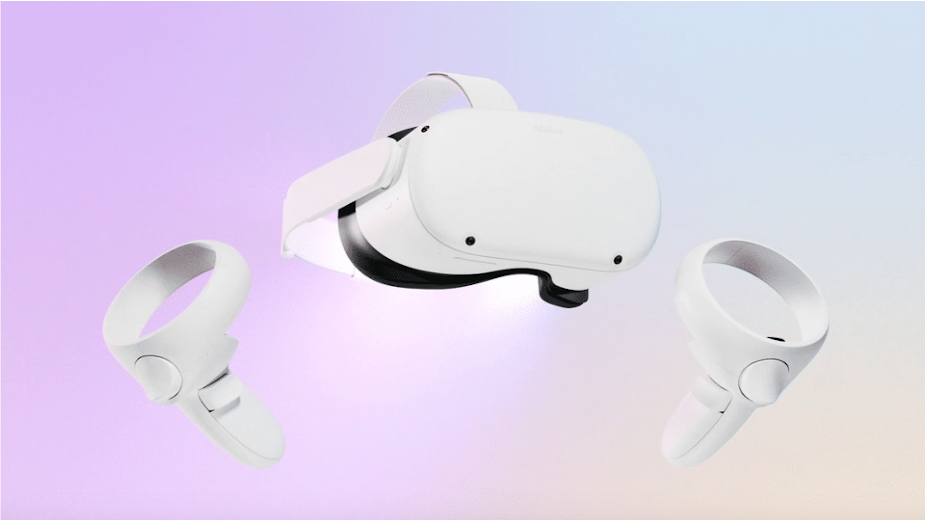
\includegraphics[width=5truecm, height=3.8truecm]{images/oculus.png}
	\caption{Oculus Quest 2 VR szemüveg}
\end{figure}


{\bf Népszerű kontrollerek:}
\begin{itemize}
\item HTC Vive : követi a kéz mozdulatot, az ujjak mozgását.
\item 3DRudder : lábbal vezérelhető.
\item SteelSeries Stratus XL: konzolhoz való kontroller kialakítású.
\end{itemize}

{\bf VR kesztyűk:}
Precízebben lehet velük követni a kéz mozgását, külön követik a ujjak mozgását.
\begin{itemize}
\item ExoGlove
\item ManusVR
\item GloveOne
\end{itemize}

\begin{figure}[htp]
    \centering
   	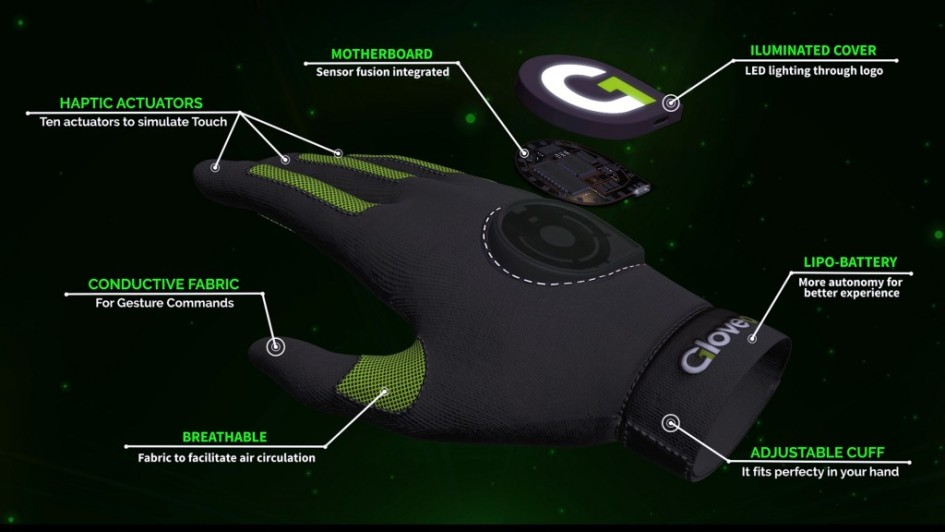
\includegraphics[width=5truecm, height=3.8truecm]{images/gloveone.jpg}
	\caption{OneGlove VR kesztyű}
\end{figure}

{\bf VR ruha:}
\begin{itemize}
\item Teslasuit
\item TactSuit
\end{itemize}

\begin{figure}[htp]
    \centering
   	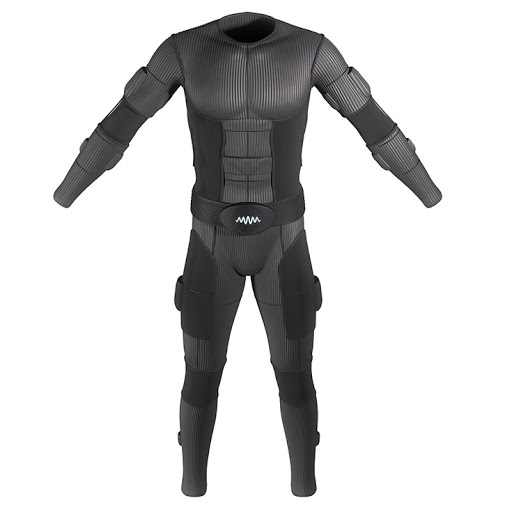
\includegraphics[width=5truecm, height=3.8truecm]{images/tesla.jpg}
	\caption{TeslaSuit VR ruha}
\end{figure}

\Section{A kiterjesztett valóság fajtái:}

\SubSection{Marker alapú (marker based)}

A markerek speciális azonosítók, amiket kamera segítségével, az AR alkalmazássalfelismerünk és a virtuális tartalmat, ami lehet egy  3D objektum például, a kamerához vizsonyított relatív pozicióba helyezzük el. 

Fontos, hogy a marker egyedi legyen és jól feismerhető a környezetben. 

Erőteljes hátránya, hogy ha a marker egy része nem látható, ha az eszköz elmodul akkor a tartalom eltűnik.
Marker lehet egyszerűbb információt hordozó bináris minta kerettel(QR-kód, ArUco marker, stb..), 2D-s kép, 3D-s objektum is.

\SubSection{Marker nélküli (markerless)}

A marker nélküli kiterjesztett valóság SLAM-et (környezet felmérése, pl. érzékeli hol a padló, a fal) használja. A tartalmat a környezethez viszonyítva lehet pozícionálni, tájolni.

Erős elönye, hogy a virtuális tartalom itt nem tűnik elmozdulás miatt, hisz nem egy adott markerhez,
hanem az egész környezethez viszonyít.

\Section{Software, SDK összehasonlítás}

\SubSection{Apple ARKit}

Az Apple ARKit az iOS operációs rendszerrel (iOS 11-től felfelé) rendelkező eszközökre (iPhone, iPad amiknek minimum A9-es processzora van) való AR alkalmazások fejlesztéséhez használható. 
Például képes: 
\begin{itemize}
\item 2D-s kép felismerésére és annak követésére.
\item 3D-s objektum felismerésére és annak elhelyezésére a térben.
\item Függöleges és vízszintes sík felismerésre.
\item Arcmozgás követésére.
\end{itemize}

\SubSection{Google ARCore}

A Google ARCore igen népszerű AR SDK, használható tabletre, telefonra való iOS és Android alkalmazások elkészítéséhez. Az alapját a pozició követés és az objektum felismerés adja.
Fontos eleme még:
\begin{itemize}
\item A fény követés a valósághűbb objektumok kialakításához.
\item Mozgás követés a telefon poziciójának felhasználásával.
\item Felismerése a  felületek méretének, elhelyezkedésének függőlegesen és vízszintesen.
\end{itemize}

\SubSection{Vuforia}

A Vuforia az egyik legnépszerűbb SDK a AR alkalmazások készítéséhez. Annak köszönhetően, hogy Unityben jól használható, lehetővé válik vele a Androidra és iOS-re való natív alkamazások készítése. Továbbá asztali gépekre is lehet vele fejleszteni, szintén a Unity-nek köszönhetően. Használható:
\begin{itemize}
\item  Kép, szöveg (csak angol természetesen), 3D-s objektumok felismerése és követése valós időben.
\item  Virtuális elemek elhelyezése a térben.  
\item  Virtuális gombok. Virtual buttons
\item  Lokalizált okklúzió felismerés a virtuális gombok használatával.
\end{itemize}
Használható számos marker típussal, marker nélkül, markerként használt objektumokkal, VuMark-kal (A VuMArk a QR-kód és kép együttese). 

\SubSection{Wikitude}

A Wikitude kíválóan alkalmazható hely-központú( WIFI vagy GPS felhasználásával) alkalmazások fejlesztésére telefonra. Továbbá népszerű a cégeknél annak köszönhetően, hogy a legrövidebb idő alatt ezzel lehet elkészíteni a vásárló-központú alkalmazásokat. Funkciói:
\begin{itemize}
\item 3D, kép felismerés és követés 
\item Helymeghatározáson alapuló AR
\item Okos szemüveg itegráció.
\end{itemize}

\SubSection{Kudan}

A Kudan egy réteget add hozzá az objektumokhoz a felismerés megkönnyítése végett. Gyors és kézenfekvő, de igényel előismereteket. Jól írányíthatók az adatok, a sebesség, az érzékenység a prokejtekből. Jól működik markerrel és anélkülis, 

\SubSection{ARToolKit}

Az ARToolKit nyílt forráskodú (elérhető GitHub-on), használható akár okosszemüvegekhez készített alkalmazások fejlesztéséhez is. Fejleszhető vele iOS, Android, Windows, MacOS és Linux platformra is alkalmazás. Rendelkezik Unity és OpenSceneGraph támogatottsággal. Támogatja az egy vagy duálkamerával való követést. Számos programozási nyelvvel hazsnáható.

\SubSection{EasyAR}

Az EasyAr ingyenes, kiváló kezdőknek., Van Pro verziója is üzleti használatra, ami extra funkciókat tartalmaz (az ingyenes verzóhoz képest sokkal hosszabb az elérhető funkciók listája.). Androidra, iOs-re és Windowsra van lehetőség fejleszteni vele.

\SubSection{MaxST}

A MaxST két SDK-ra válik szét: egy a 2D kép felismeréshezés egy a 3D objektumokhoz. Felismeri a függőleges és vízszintes síkokat, akár több objektumot is képes egyszerre követni, alkalmas QR-kód és vonalkód szkenneléshez.

\SubSection{Pikkart AR SDK}

A Pikkart SDK segítségével egyedi, funkció gazdag, felhasználóbarát alkallmazásokat lehet készíteni. Könnyű fejlesztési folyamatot biztosít.
\SubSection{AR.js}

Az AR.js egy JavaScript alapú, nyíltforráskodú AR SDK. Böngészőben használható Ar alklamazások készítéséhez használható, nem igényel telepítést. Minden mobil platformon képes futni az ezzel az SDK-val készített alkalmazás.

\SubSection{További API-k}

\begin{itemize}
\item ARLab
\item Onirix
\item DeepAR
\item MixedReality Toolkit (Hololens)
\item Xzimg
\item DroidAR
\item HP Reveal Studio
\item BlippBuilder
\end{itemize}

\Section{Unity}

A Unity egy  olyan cross-platform játék motor, amellyel lehetőségünk van Windowsra, Linuxra, Mac OS-re, iOS-re, Androidra, valamint Wii-re és más jéték konzolokra fejleszteni.

Van üzleti és személyi változata is. Bizonyos keretek alatt ingyenes lehet a cégeknek is, nem csak a magánszemélyeknek.

A dolgozat elkésztéséhez először Unityt akartam használni, azonban több probléma is felmerült. 

Túlságosan erőforrás igényes, speciális eszközöket igényelnek a kiprobálható demók (pl. VR szemüveg), nem találtam megfelelő leírásokat a példákhoz és a verziók közötti váltás is problémát okozott.

Ezért a dolgozat OpenCV, OpenGL és python segytségével készítettem el.
